%!TEX root = ../article.tex

% \listoftodos

%1
\levelA{\label{chap:introduction}Introduction}
\input{content/1-introduction.tex}

    %\levelB{Motivation}
    %from pep 1, paragrafo 1
In a forensic context, file recovery is a frequent task that can be motivated by several situations, like physical media malfunction, intentional attempt to hide data, and the need to access deleted or older versions of files. When the filesystem no longer provides the physical location of a file on the media, data carving is often the only procedure capable of retrieving this content.

%from pep 1, paragrafo 2
Data carving is a forensic process that attempts to recover files without previous information of where the file starts or ends \cite{garfinkel_carving_2007}.
To accomplish this, a program has to analyze a source of raw data, searching for patterns indicating a known file type and making attempts to locate and reconstruct each of its constituent parts.

%from pep 1, paragrafo 2b
That process commonly disregards the filesystem \cite{veenman_statistical_2007}, being able to recover deleted files from unallocated areas, but faces the problem of fragmentation \cite{veenman_statistical_2007}  \cite{pal_evolution_2009}: in many cases, files are not written sequentially on disk and deleted files may have missing parts.

This procedure is frequently used in forensic environments, but it may also be beneficial in other areas, such as reverse engineering, network traffic analysis, and data mining.

This observation is related to the fact that many types of data sources contain embedded files. Therefore, they may be used as input to a data carving process. This includes network traffic, memory dumps, hard drive images, and files containing other files.


    % \input{content/1.1b-example.tex}
    % \input{content/1.1c-datacarvingclasses.tex}

    

% Misclassification analysis should play a prominent role in published classification research. In the past, researchers have focused on building classifiers without discussing classification errors, which significantly degrades the contribution to the body of knowledge. Such discussion helps us explain classifier performance 

% The results show
% the classifier more accurately classifies low entropy data, similar to past research findings.


% Scalability could also be improved via a hierarchical classi-
% fication approach, since it reduces the number of classes. In a
% hierarchical classification approach, a file fragment is classified
% into one of several large categories and then further classified
% into a specific type within the category, which may not even be
% needed in all cases.

    %\levelB{Research questions}

    \subsection{Research question}
% This work compares the use of Multilayer Perceptrons (MLP), Convolutional Neural Networks (CNN) and Long Short-Term Memory (LSTM), and combinations of those types of networks, to perform file fragment classification, which is the first step of the data carving process, identification, answering the following initial questions:

The study of Beebee et al. \cite{beebe_sceadan:_2013} is one of the best works on file fragment classification: it emphasized the problem of multiple data types in a file type, achieved high accuracy using a large amount of file types, made their source code available, suggested hierarchical classification as a way to improve scalability, suggested that misclassification analysis should play a prominent role in classification research, endorsed that high entropy file types tend to have a lower classification accuracy, and briefly mentions that the number of classes should be taken in consideration when comparing accuracy of different studies.

This research addresses specifically the last item in the list, the influence of number of classes in accuracy, but the two previous items, misclassification analysis and high entropy, are also part of the discussion. Although is intuitive that a higher number of classes should have an influence on the results of a file fragment classifier, the issue, considering the carving problem perspective, wasn't formally studied yet. Thus, the following initial question is proposed:

%from pep 4.1
\begin{enumerate}[itemindent=\parindent,label=\textbf{Q\arabic*.}]

% Then, the influence of the number of classes on the accuracy of the resulting models is briefly explored.
    \item How does the accuracy of neural network models change relative to the number of classes?

\end{enumerate}

% In this work, only neural networks are implemented, but other machine learning approaches exist, like Support Vector Machines (SVM) and k-Nearest Neighbors (kNN). This choice of restriction was motivated by the success that deep neural networks have shown in other fields, like image classification and speech recognition.
% The flexibility of neural networks to combine different types of layers is also important, as it is a core characteristic being explored in this research.

% Two sets of experiments were conducted. In the first set, the initial 512 bytes of a file is used as input to the tested neural network, whose task is to predict the file type. The second set is similar, but the 512 bytes fragment is extracted from a random position of the file, which is a more difficult task as it cannot depend on header patterns.

    %\levelB{Overview}

    % \subsection{Outline}
% providing an overview of the dissertation or report structure

The remainder of this document is organized as follows.
% \todo{check later}
    Section 2 analyses current researches on file fragment classification using the Govdocs1 dataset. 
    Section 3 describes the proposed method.
    Section 4 presents the results.
    Section 5 discusses the results, including suggestions for future work.
    Section 6 presents the conclusion.



%3
\levelA{Related work}
\input{content/2-relatedwork.tex}
    \label{sec:relatedwork}
    % \levelB{From PEP}
    This related work summary focuses on studies on file fragment classification that used the Govdocs1 dataset\cite{garfinkel_bringing_2009}.

The early studies on data carving used private datasets, making it difficult to compare the results of different studies. In 2009, Garfinkel et al. \cite{garfinkel_bringing_2009} published the Govdocs1 dataset with 1 million files (a small amount of those files were removed later, for legal caution). While some of the later works on the field still use private datasets, the Govdocs1 dataset has become the most used choice in studies related to data carving.

Depending on the objective, the focus of each study may either be whole file classification or file fragment classification. Whole file classification is generally an easier task because most file types, even those with high entropy and low compression rates, have well-structured headers, with easily recognizable patterns.

Most of the early work on this field used some form of dimensionality reduction on the input data before performing classification, as byte frequency distribution, compression rate, and various statistical techniques. The usage of raw bytes as input is recently becoming more popular, especially in studies applying machine learning techniques, which seems to be a rising trend in the last ten years.


Axelsson \cite{axelsson_normalised_2010}
used the normalized compression distance as an input feature to a kNN algorithm,
picking pairs of 512 bytes fragments, compressing them with the bzip2 algorithm
and comparing the length of the results.
% He used 28 file types from the Govdocs1 dataset
% : pdf, html, jpg, text, doc, xls, ppt, xml, gif, ps, csv, gz, eps, png, swf, pps, sql, java, pptx, docx, ttf, js, pub, bmp, xbm, xlsx, jar, and zip.
He got an average accuracy of around 34\% using 28 file types.

% Gopal et al. \cite{gopal_statistical_2011}  \todo{describe approach}. They used RDC

Fitzgerald et al. \cite{fitzgerald_using_2012}  
used an SVM classifier with various statistical measures as input features, including unigram and bigram histogram counts, Shannon entropy, and compression length.
% They used 24 file types from the the Govdocs1 dataset, 
% : pdf, ppt, txt, jpg, doc, xls, ps, html, gz, xml, pps, csv, gif, swf, png, pptx, rtf, sql, docx, bmp, zip, java, xlsx, and tex, 
Omitting first and last fragments of each file,
They got an average accuracy of 49.1\% using 24 file types.

Beebe et al. \cite{beebe_sceadan:_2013}
compared various measures of complexity and byte frequency distributions of 512 bytes fragments as input features to an SVM algorithm.
They used 8 data types, txt, base64, base85, urlencoded, fat fs data, ntfs fs data, ext fs data, aes256, and
30 file types
% , jpg, gif, bmp, png, tif, pdf, ps, zip, bzip2, gzip, doc, docx, xls, xlsx, ppt, pptx, wmv, mp3, mp4, avi, flv, m4a, java, js, html, xml, json, csv, css, and log, 
from the Govdocs1 dataset and some other sources (19 are at least partially from the Govdocs1 dataset).
They got an average accuracy of 73.4\% combining unigram and bigrams as input features.

Chen et al. \cite{chen_file_2018}
used a Convolutional Neural Network (CNN) with 5 convolutional layers and 3 fully connected layers to classify fragments of 4096 bytes, converting each fragment into a 64x64 grayscale picture.
% They used 16 file types from the Govdocs1 dataset
% : csv, doc, docx, gif, gz, html, java, jpg, log, pdf, png, ppt, rtf, text, xls, xml.
They got an average accuracy of 70.9\% using 16 file types.

Hiester \cite{hiester_file_2018} apparently was the first to utilize an LSTM network to perform file fragment classification. He compared results using three types of neural networks: feedforward, convolutional, and long short-term memory. He used four file types from the Govdocs1 dataset.
% : csv, xml, jpg and gif. 
Each bit of a 512-byte fragment was translated into two features, resulting in 8192 features per block (512 * 8 * 2). The first and last sectors of each file in the training set were discarded. In the experiments, the datasets were limited to one gigabyte to fit on memory. He got an average accuracy of 98\% using an LSTM network, 73\% using CNN, and 76\% using MLP.

Wang et al. \cite{wang_sparse_2018} 
used sparse dictionaries for n-grams to extract features of 512 bytes fragments, using this as input to an SVM classifier.
% They used 18 file types from the Govdocs1 dataset
% : csv, doc, docx, gif, gz, html, jpg, pdf, png, ppt, pptx, ps, rtf, swf, txt, xls, xlsx, and xml.
They got an average accuracy of 61.3\% using 18 file types.

Wang et al. \cite{wang_file_2018}  
compared CNN, SVM, kNN, and XGboost, with fragments of different sizes, converting each byte to a 256 length vector (one-hot encoding). The CNN combined 3 parallel convolutional layers of widths 4, 8, and 16.
They used 20 file types from the Govdocs1 dataset.
% : csv, doc, html, pdf, gif, jpg, dbase3, f, txt, swf, ps, java, log, xml, xls, ppt, gz, unk, rtf, and png.
Using the CNN, they got an average accuracy of around 68\% with 512 bytes fragments, and around 78\% with 4096 bytes fragments.

Vulinović et al. \cite{vulinovic_neural_2019}
compared a CNN with MLP, using 512 raw bytes as the CNN input, and byte histograms as input to the MLP.
% They used 18 file types from the Govdocs1 dataset
% : csv, doc, docx, gif, gz, html, jpg, pdf, png, ppt, pptx, ps, rtf, swf, txt, xls, xlsx, and xml.
Using 18 file types, they got a macro average f1 score of 61\% using CNN and 81\% using MLP.

Table \ref{tab:datacarvingstudies} summarizes 
the results of file fragment classification studies using Govdocs1 dataset and table \ref{tab:studiesfiletypes}
lists the file types used in each study.

\begin{table*}[!ht]
\caption{\label{tab:datacarvingstudies}File fragment classification studies using the Govdocs1 dataset}
\resizebox{\linewidth}{!}{%
\begin{tabular}{|l|l|l|l|l|l|l|l|l|l|l|}
\hline
Study                                          & SVM & kNN & NN   & Dataset       & Raw   & Fragment & Number   & Accuracy   & F1-score  \\
                                               &     &     &      &               & bytes & size     & of types &            &           \\ \hline
Axelsson \cite{axelsson_normalised_2010}       &     & x   &      & Govdocs1      & No    & 512      & 28       & 34\%       &           \\ \hline
Fitzgerald et al. \cite{fitzgerald_using_2012} & x   &     &      & Govdocs1      & No    & 512      & 24       & 49\%       & 48\%      \\ \hline
Beebe et al. \cite{beebe_sceadan:_2013}        & x   &     &      & Govdocs1 +    & No    & 512      & 38       & 73\%       &           \\
                                               &     &     &      & other sources &       &          &          &            &           \\ \hline
Hiester \cite{hiester_file_2018}               &     &     & MLP  & Govdocs1      & Yes   & 512      & 4        & 77\%       &           \\
                                               &     &     & CNN  &               &       &          &          & 73\%       &           \\
                                               &     &     & LSTM &               &       &          &          & 98\%       &           \\ \hline
Chen \cite{chen_file_2018}                     &     &     & CNN  & Govdocs1      & Yes   & 4096     & 16       & 71\%       &           \\ \hline
Wang \cite{wang_sparse_2018}                   & x   &     &      & Govdocs1      & Yes   & 512      & 18       & 61\%       & 61\%      \\ \hline
Wang \cite{wang_file_2018}                     &     &     & CNN  & Govdocs1      & Yes   & 512      & 20       & 68\%       &           \\
                                               &     &     &      &               &       & 4096     &          & 78\%       &           \\ \hline
Vulinovic \cite{vulinovic_neural_2019}         &     &     & MLP  & Govdocs1      & Yes   & 512      & 18       &            & 81\%      \\
                                               &     &     & CNN  &               &       &          &          &            & 61\%      \\ \hline
\end{tabular}}
\end{table*}

\begin{table}[!ht]
    \centering
    \caption{The Govdocs1 dataset and file types used in each study}
    \label{tab:studiesfiletypes}
\footnotesize
\begin{tabular}{|l|l|l|l|l|l|l|l|l|l|l|l|}
\hline
Extension & Number of files & Number of blocks
                                            & \rotatebox{90}{this study}
                                                & \rotatebox{90}{Axelsson \cite{axelsson_normalised_2010}}
                                                    & \rotatebox{90}{Fitzgerald et al. \cite{fitzgerald_using_2012}}
                                                        & \rotatebox{90}{Beebe et al. \cite{beebe_sceadan:_2013}}
                                                            & \rotatebox{90}{Hiester \cite{hiester_file_2018}}
                                                                & \rotatebox{90}{Chen \cite{chen_file_2018}}
                                                                    & \rotatebox{90}{Wang \cite{wang_sparse_2018}}
                                                                        & \rotatebox{90}{Wang \cite{wang_file_2018}}
                                                                            & \rotatebox{90}{Vulinovic \cite{vulinovic_neural_2019}}
                                                   \\ \hline
                                                      \hline
pdf       & 231232          & 268071071     & x & x & x & x &   & x & x & x & x   \\ \hline
html      & 214568          & 25710908      & x & x & x & x &   & x & x & x & x   \\ \hline
jpg       & 109233          & 73242253      & x & x & x & x & x & x & x & x & x   \\ \hline
txt       & 78286           & 99435540      & x &   & x & x &   &   & x & x & x   \\ \hline
doc       & 76616           & 60654930      & x & x & x & x &   & x & x & x & x   \\ \hline
xls       & 62635           & 58718224      & x & x & x & x &   & x & x & x & x   \\ \hline
ppt       & 49702           & 251210471     & x & x & x & x &   & x & x & x & x   \\ \hline
gif       & 36302           & 5962516       & x & x & x & x & x & x & x & x & x   \\ \hline
xml       & 33458           & 16954875      & x & x & x & x & x & x & x & x & x   \\ \hline
ps        & 22015           & 56547464      & x & x & x & x &   &   & x & x & x   \\ \hline
csv       & 18360           & 6843009       & x & x & x & x & x & x & x & x & x   \\ \hline
gz        & 13725           & 17748905      & x & x & x & x &   & x & x & x & x   \\ \hline
log       & 9976            & 8467819       & x &   &   & x &   & x &   & x &     \\ \hline
eps       & 5191            & 5756138       & x & x &   &   &   &   &   &   &     \\ \hline
unk       & 5186            & 2983922       &   &   &   &   &   &   &   & x &     \\ \hline
png       & 4125            & 2207489       & x & x & x & x &   & x & x & x & x   \\ \hline
swf       & 3476            & 3798321       & x & x & x &   &   &   & x & x & x   \\ \hline
dbase3    & 2601            & 38972         & x &   &   &   &   &   &   & x &     \\ \hline
pps       & 1619            & 7432480       & x & x & x &   &   &   &   &   &     \\ \hline
rtf       & 1125            & 958239        & x &   & x &   &   & x & x & x & x   \\ \hline
kml       & 993             & 309422        & x &   &   &   &   &   &   &   &     \\ \hline
kmz       & 943             & 549462        & x &   &   &   &   &   &   &   &     \\ \hline
text      & 839             & 1527118       &   & x &   &   &   & x &   &   &     \\ \hline
hlp       & 659             & 8692          & x &   &   &   &   &   &   &   &     \\ \hline
f         & 602             & 94543         & x &   &   &   &   &   &   & x &     \\ \hline
sql       & 462             & 244634        & x & x & x &   &   &   &   &   &     \\ \hline
wp        & 364             & 87643         & x &   &   &   &   &   &   &   &     \\ \hline
dwf       & 299             & 85500         & x &   &   &   &   &   &   &   &     \\ \hline
java      & 292             & 14530         & x & x & x & x &   & x &   & x &     \\ \hline
pptx      & 215             & 1151796       & x & x & x & x &   &   & x &   & x   \\ \hline
% fits      & 182             & 678128        &   &   &   &   &   &   &   &   &     \\ \hline
% tmp       & 180             & 28426         &   &   &   &   &   &   &   &   &     \\ \hline
tex       & 163             & 10520         &   &   & x &   &   &   &   &   &     \\ \hline
docx      & 163             & 65969         &   & x & x & x &   & x & x &   & x   \\ \hline
% troff     & 110             & 8020          &   &   &   &   &   &   &   &   &     \\ \hline
bmp       & 72              & 62686         &   & x & x & x &   &   &   &   &     \\ \hline
% sgml      & 62              & 44138         &   &   &   &   &   &   &   &   &     \\ \hline
% gls       & 60              & 517           &   &   &   &   &   &   &   &   &     \\ \hline
pub       & 55              & 1421          &   & x &   &   &   &   &   &   &     \\ \hline
xlsx      & 37              & 12910         &   & x & x & x &   &   & x &   & x   \\ \hline
% fm        & 25              & 6717          &   &   &   &   &   &   &   &   &     \\ \hline
zip       & 10              & 31525         &   & x & x &   &   &   &   &   &     \\ \hline
ttf       & 10              & 1540          &   & x &   &   &   &   &   &   &     \\ \hline
xbm       & 8               & 578           &   & x &   &   &   &   &   &   &     \\ \hline
% wk1       & 7               & 6493          &   &   &   &   &   &   &   &   &     \\ \hline
% sys       & 7               & 15            &   &   &   &   &   &   &   &   &     \\ \hline
% ileaf     & 4               & 1656          &   &   &   &   &   &   &   &   &     \\ \hline
% exported  & 3               & 324           &   &   &   &   &   &   &   &   &     \\ \hline
% data      & 3               & 1733          &   &   &   &   &   &   &   &   &     \\ \hline
% odp       & 2               & 2384          &   &   &   &   &   &   &   &   &     \\ \hline
% mac       & 2               & 0             &   &   &   &   &   &   &   &   &     \\ \hline
% lnk       & 2               & 2             &   &   &   &   &   &   &   &   &     \\ \hline
js        & 2               & 36            &   & x &   &   &   &   &   &   &     \\ \hline
% g3        & 2               & 498           &   &   &   &   &   &   &   &   &     \\ \hline
% chp       & 2               & 73            &   &   &   &   &   &   &   &   &     \\ \hline
% 123       & 2               & 434           &   &   &   &   &   &   &   &   &     \\ \hline
% wk3       & 1               & 229           &   &   &   &   &   &   &   &   &     \\ \hline
% vrml      & 1               & 660           &   &   &   &   &   &   &   &   &     \\ \hline
% squeak    & 1               & 25354         &   &   &   &   &   &   &   &   &     \\ \hline
% py        & 1               & 480           &   &   &   &   &   &   &   &   &     \\ \hline
% pst       & 1               & 20            &   &   &   &   &   &   &   &   &     \\ \hline
% icns      & 1               & 0             &   &   &   &   &   &   &   &   &     \\ \hline
% bin       & 1               & 7             &   &   &   &   &   &   &   &   &     \\ \hline
\end{tabular}
\end{table}


% % In 2014, 
% Alamri and Allen \cite{alamri_taxonomy_2014} created a taxonomy of file type identification techniques, grouped by the following broad categories: statistical learning, frequency distribution, statistical analysis, and detection of file fragments. The statistical learning category is subdivided in supervised and unsupervised leaning. The supervised learning techniques are Support Vector Machine (SVM), k-Nearest Neighbor (kNN), and Neural Network (NN). According to this taxonomy study, SVM is used in \cite{ahmed_fast_2011}, \cite{amirani_feature-based_2013}, \cite{beebe_sceadan:_2013}, \cite{fitzgerald_using_2012}, \cite{gopal_statistical_2011}, and \cite{sportiello_context-based_2012}, kNN is used in \cite{ahmed_fast_2011} and \cite{gopal_statistical_2011}, while neural networks are used in \cite{ahmed_fast_2011}, \cite{ahmed_content-based_2010}, \cite{amirani_new_2008}, \cite{amirani_feature-based_2013}, and \cite{penrose_approaches_2013}.

% % In 2018, 
% Ali et al. \cite{ali_review_2018} reviewed digital forensics methods for JPEG file carving. JPEG is mentioned in that paper as a common focus among data carving studies. Only some of the analyzed studies utilize some machine learning technique:
% neural networks are used in \cite{xu_reassembling_2009} and \cite{amirani_feature-based_2013},
% SVM is used in \cite{qiu_new_2014}, \cite{zhang_svm_2016}, and \cite{sportiello_file_2011},
% kNN is used in \cite{axelsson_normalised_2010},
% and Extreme Learning Machine (ELM) is used in \cite{zhang_svm_2016} and \cite{ali_classification_2018}.


% Other works studying machine learning techniques applied to data carving include: \cite{luigi_file_2011} using SVM,
% and Conti et al. \cite{conti_automated_2010} using kNN to classify low-level primitive types, like ASCII text, compressed data, bitmap, and encoded schemes.

% According to Ali et al. \cite{ali_review_2018}, artificial intelligence techniques are found to be not fully utilized in this field.

% In 2005, 
% Dunhan et al. \cite{dunham_classifying_2005} have successfully identified file type of encrypted files. First, they used a two-level neural network to identify files encrypted with the same key. Then, within each group of files, they used a three-level neural network to identify file types, using file deltas created with exclusive-or as input to the neural network. The samples included the beginning of the files.

% In 2007, 
% Harris \cite{harris_using_2007} described the attempt to use a neural network in data carving. He compared the use of bytes frequency distribution against the use of the raw bytes. Even using the begging of files, the achieved accuracy was lower than 60\%. The use of floats to represent bytes must have contributed to those low results.

% In 2008, 
% Amirami et al.  \cite{amirani_new_2008} used Principal Component Analysis (PCA) as input for a 5 layer feed-forward auto-associative unsupervised neural network to do feature extraction and a 3 layer Multi Layer Perceptron (MLP) to perform classification.  They used byte frequency distribution of the entire file as initial features. 
% In 2009, 
% Xu and Dong \cite{xu_reassembling_2009}, used a neural network as a cluster reassembling technique for JPEG image fragments.
% network structure not detailed

% In 2010, 
% Ahmed et al. \cite{ahmed_content-based_2010}, used byte frequency distribution of entire files as input to a neural network that performed file type classification. They used a similar approach in their later work \cite{ahmed_fast_2011}, but compared with features taken from fragments of files. These fragments included the beginning of the files.

% In 2013, 
% Penrose et al. \cite{penrose_approaches_2013}, using compression rate as the input to a neural network to distinguish between compressed and encrypted files;
% In 2014, 
% Maslim et al. \cite{maslim_distributed_2014}, using Principal Component Analysis (PCA) of byte frequency distribution as input to a Gene Regulatory Engine (GRE) and a Distributed Adaptative Neural Network (DANN).


    % \levelB{Current data carving tools}
    % \input{content/2.2-datacarvingtools.tex}
    % \levelB{Data carving challenges}
    % %%%%%%%%%%%%%%%%%%%%%%%%%%%%%%%%%%%%%%%%%%%%%%%%
% indicating a problem, controversy or a knowledge gap in the field of study

% identification
% validation
% fragmentation
%from pep 4, paragrafo 5
Each of the steps cited by Ali et al. \cite{ali_review_2018} for the data carving process deals with a main challenge. The identification step is responsible for classifying the file type. The quantity and diversity of file types, together with the accuracy and precision of the results, are the main challenges in identification. The second step, validation, also deals with classification, but it is a complementary step to the previous one to reduce false positives, often using a different technique. For that reason, validation challenges are similar to the identification ones. The last step, reassembling, has fragmentation as its main challenge.

% - more file types
% - reassembling
% - new carvers easier
%from pep 4, paragrafo 4
The work of Hiester \cite{hiester_file_2018} has shown that LSTM neural networks have good potential in the data carving field. But, as happens with studies applying LSTM models to speech recognition, where many researchers have contributed with different models, adjustments, modifications, and innovations, also in the field of data carving field it is important to further advance the research. Important aspects that require attention include support for a wider range of file types, handle fragmentation through reassembling, and make the task of supporting the carving of a new file type easier.

% datasets and file structures

% challenge: reveal structures in the file
% from pep 4, paragrafo 6
% In the current proposal, a new type of challenge is introduced. Instead of using previous knowledge of the file structure to improve carving results, \textbf{would be possible to do the inverse and use insights from the carving process to reveal structures in the file?}

% challenge: reveal structures in the file
%from pep 4, paragrafo 7
% For example, suppose a file has a fixed size field, a 32 bit unsigned integer representing a datetime value. 
% For that type of field, the insight may come in the form of an expected range. Still using the datetime example, a possible outcome would be the observation that a certain kind of file always presents that field value inside some range, that coincides with a range often observed in datetime fields. That does not prove the unknown field to be a datetime but suggests that direction.

% challenge: reveal structures in the file
%from pep 4, paragrafo 8
% Few structures are so simple as a group of fixed sized fields. It is very common, for example, to use a field to specify the length of the next field. Another type of complexity increase occurs when the value of a field establishes which specification should be used in the remaining of the file, changing which fields should be expected next.

% challenge: reveal structures in the file
% %from pep 4, paragrafo 9
% The greater the complexity of an unknown file structure is, the more difficult it is to unravel its specification, but also the more useful it is to count with tools that automatize that task. Otherwise, the only option is to manually write the specification or the parser, possibly relying on reverse engineering techniques.

% challenge: reveal structures in the file
%from pep 4, paragrafo 10
% The direct utility of the discovery of file type structures is the extraction of values from its fields. This information has value for itself, but could also be used to improve validation and even reassembling.

% challenge: datasets
%from pep 4, paragrafo 11
% Another concern that can be explored and is pertinent to possibly all of the previous studies combining neural networks and data carving is that their datasets and results may not reflect the same situations that would be faced on a real forensic scenario, where the distribution of file types may be different and the occurrence of unknown and untreated formats may be frequent. Therefore, more realistic datasets are important to improve research validation. 
%%%%%%%%%%%%%%%%%%%%%%%%%%%%%%%%%%%%%%%%%%%%%%%%


    \levelB{Neural networks researches in data carving}
    
%from pep 2.1, paragrafos 12, 13
Amirani et al.  \cite{amirani_new_2008} appear to be the first 
to provide a viable alternative to classical data carving tools using a neural network approach. Two previous works were found using neural networks with data carving related goals, by Dunham et al. \cite{dunham_classifying_2005} and Harris \cite{harris_using_2007}, but the first worked with encrypted files only and the second did not achieve good results.

%from pep 2.1, paragrafos 14
Amirani et al.  \cite{amirani_new_2008} used Principal Component Analysis (PCA) as input for a 5 layer feed-forward auto-associative unsupervised neural network to do feature extraction and a 3 layer Multilayer Perceptron (MLP) to perform classification. They used a similar approach in 2013 \cite{amirani_feature-based_2013}.
\sigla{PCA}{Principal Component Analysis}
\sigla{MLP}{Multilayer Perceptron}

%from pep 2.1, paragrafos 16,17,18
Other works were found applying neural networks to perform data carving, also using some form of dimensionality reduction as PCA. Ahmed et al. \cite{ahmed_content-based_2010}\cite{ahmed_fast_2011} used byte frequency, 
Penrose et al. \cite{penrose_approaches_2013} used compression rate,
and Maslim et al. \cite{maslim_distributed_2014} used PCA, as did Amirani et al.  \cite{amirani_new_2008}.

%from pep 2.1, paragrafos 15
Xu and Dong \cite{xu_reassembling_2009} used a neural network as a cluster reassembling technique for JPEG image fragments.

%from pep 2.1, paragrafos 19
Hiester \cite{hiester_file_2018} apparently was the first to not resort to dimensionality reduction and also the first to utilize an LSTM network to perform file fragment classification. He compared results using three types of neural networks: feedforward, convolutional, and long short-term memory. The goal was to classify the data type of individual sectors (512 bytes), considering four file types: CSV, XML, JPG and GIF.

% Table \ref{tab:datacarvingstudies} summarizes the  machine learning techniques used in each data carving study.
% \input{content/tables/3.3-table-studies.tex}

%2
% \levelA{\label{chap:background}Some artificial neural networks}
% \input{content/3-background.tex}
%     \levelB{\label{sec:feedforward}Multilayer Perceptron}
%     \input{content/3.2-feedforward.tex}
    
%     \levelB{\label{sec:conv}Convolutional neural network}
%     \input{content/3.3-conv.tex}
    
%     % \levelB{\label{sec:rnn}Recurrent Neural Network}
%     % \input{content/3.4-rnn.tex}
    
%     \levelB{\label{sec:lstm}Long Short-Term Memory}
%     \input{content/3.5-lstm.tex}

%4
\levelA{\label{chap:experiments}Proposed method}
This study describes how does the accuracy of neural network models change relative to the number of classes in the dataset.

\levelB{Dataset}
This study uses the Govdocs1 dataset \cite{garfinkel_bringing_2009}, which was fully downloaded and its files were grouped by extension. This dataset has files with 63 different extensions. The 33 extensions with less than 200 files were discarded. The  ``text'' and ``unk'' extensions were discarded because files with these extensions use multiple formats and they do not correspond to a single file type. From the remaining 28 extensions, listed in table \ref{tab:studiesfiletypes}, 200 files of each were randomly selected, 100 to use in the training dataset and 100 to use in the validation dataset.

\begin{table}[!ht]
    \centering
    \caption{Govdocs1 dataset}
    \label{tab:govdocs1}
\begin{tabular}{|l|l|l|}
\hline
Extension & Number of files & Number of blocks \\ \hline
                                                  \hline
pdf       & 231232          & 268071071    \\ \hline
html      & 214568          & 25710908     \\ \hline
jpg       & 109233          & 73242253     \\ \hline
txt       & 78286           & 99435540     \\ \hline
doc       & 76616           & 60654930     \\ \hline
xls       & 62635           & 58718224     \\ \hline
ppt       & 49702           & 251210471    \\ \hline
gif       & 36302           & 5962516      \\ \hline
xml       & 33458           & 16954875     \\ \hline
ps        & 22015           & 56547464     \\ \hline
csv       & 18360           & 6843009      \\ \hline
gz        & 13725           & 17748905     \\ \hline
log       & 9976            & 8467819      \\ \hline
eps       & 5191            & 5756138      \\ \hline
% unk       & 5186            & 2983922      \\ \hline
png       & 4125            & 2207489      \\ \hline
swf       & 3476            & 3798321      \\ \hline
dbase3    & 2601            & 38972        \\ \hline
pps       & 1619            & 7432480      \\ \hline
rtf       & 1125            & 958239       \\ \hline
kml       & 993             & 309422       \\ \hline
kmz       & 943             & 549462       \\ \hline
% text      & 839             & 1527118      \\ \hline
hlp       & 659             & 8692         \\ \hline
f         & 602             & 94543        \\ \hline
sql       & 462             & 244634       \\ \hline
wp        & 364             & 87643        \\ \hline
dwf       & 299             & 85500        \\ \hline
java      & 292             & 14530        \\ \hline
pptx      & 215             & 1151796      \\ \hline
% fits      & 182             & 678128       \\ \hline
% tmp       & 180             & 28426        \\ \hline
% tex       & 163             & 10520        \\ \hline
% docx      & 163             & 65969        \\ \hline
% troff     & 110             & 8020         \\ \hline
% bmp       & 72              & 62686        \\ \hline
% sgml      & 62              & 44138        \\ \hline
% gls       & 60              & 517          \\ \hline
% pub       & 55              & 1421         \\ \hline
% xlsx      & 37              & 12910        \\ \hline
% fm        & 25              & 6717         \\ \hline
% zip       & 10              & 31525        \\ \hline
% ttf       & 10              & 1540         \\ \hline
% xbm       & 8               & 578          \\ \hline
% wk1       & 7               & 6493         \\ \hline
% sys       & 7               & 15           \\ \hline
% ileaf     & 4               & 1656         \\ \hline
% exported  & 3               & 324          \\ \hline
% data      & 3               & 1733         \\ \hline
% odp       & 2               & 2384         \\ \hline
% mac       & 2               & 0            \\ \hline
% lnk       & 2               & 2            \\ \hline
% js        & 2               & 36           \\ \hline
% g3        & 2               & 498          \\ \hline
% chp       & 2               & 73           \\ \hline
% 123       & 2               & 434          \\ \hline
% wk3       & 1               & 229          \\ \hline
% vrml      & 1               & 660          \\ \hline
% squeak    & 1               & 25354        \\ \hline
% py        & 1               & 480          \\ \hline
% pst       & 1               & 20           \\ \hline
% icns      & 1               & 0            \\ \hline
% bin       & 1               & 7            \\ \hline
\end{tabular}
\end{table}


\levelB{Hardware}
The experiments did not take advantage of GPU acceleration and were  conducted on a single computer with 256GB of RAM and with 2 Intel\textregistered Xeon\textregistered E5-2630 v2 processors, with 6 cores each, with 2 hyper-threads per core, or 24 hyper-threads in total. 


\levelB{Software}
The main software and frameworks used to build the experiments were Python 3.6, Jupyter notebook, Tensorflow 1.14.0, Keras 2.2.4-tf, and Fedora Linux 27.

% repository
The source code for the experiments is available at \sloppy\url{http://github.com/atilaromero/randomness-experiments}.

\levelB{Objective}
In the preliminary tests, it was observed that achieving 0.6 accuracy on file fragment classification using 28 classes was a difficult task to the considered models. In other studies results \cite{hiester_file_2018} \cite{sportiello_context-based_2012} \cite{amirani_feature-based_2013} \cite{maslim_distributed_2014} and on initial tests, the achieved accuracy for small number of classes was considerably higher. Hiester \cite{hiester_file_2018}, for instance, achieves an accuracy of 98\% using four classes.


\levelB{Dataset}
Several independent models were trained with 2 to 28 extensions from the Govdocs1 dataset. For each number in the range 2 to 28, a random subset of extensions was selected to compose the dataset. Each extension has 200 file samples, half placed in the training dataset and half in the validation dataset. Each dataset was used to train a new model, that should distinguish between the selected subset of extensions in that filtered dataset. This process was repeated five times.

In addition to this sampling of extensions using different quantities of classes, all 378 combinations of pairs of extensions were compared. Each pair was used to compose a dataset and to train a new model for each one, using the same process described in the previous paragraph.

Given the number of different models trained (135 for the N classes phase and 378 for the pairs), it was important to use a model architecture that had a fast training time. Models trained with the chosen architecture took about 10 minutes to train. Without this short training period, this study would not be feasible.

\levelB{Sampling}
To select a sample instance from the Govdocs1 dataset, first a random file is selected among those available, without replacement. Then, a block from this file is randomly selected. After all files have participated in the process, the process may be repeated as long as necessary. This way, all files are considered and the classes are easily balanced.
This contrasts with the sampling technique applied in other works, where all the sectors are grouped before sampling, which may lead to an imbalance between classes.

\levelB{Inputs}
%one-hot
The input features of the network for each instance is a 512x256 matrix representing only one block of 512 bytes of a random file of the dataset. Each of the 512 bytes is one-hot encoded, meaning that its value is converted into a vector with 256 elements, with only one of them set to 1, corresponding to the value of the byte, while the others are set to zero. A batch size of 100 was used, with 28 steps per epoch.

\levelB{Outputs}
The output of the network for a given instance is a vector with a size equal to the number of classes, subjected to a softmax function, which applies the exponential function on the vector and then normalizes it. Each value will represent the predicted probability that the instance belongs to a specific class.

\levelB{Model}
Before doing the procedures here described, 14 combinations of types of layers were compared, using LSTM, convolutional, and fully-connected layers. For each combination, some variations in parameters were also experimented with. This led to the three-layer model used in this research. The first is a convolutional layer with 256 output units, a window of size 16, and a stride of 16. The second is a LSTM layer of 128 units. The last is a fully-connected layer where the number of output units match the number of classes of the input dataset.

%optimization
All the trainings used the Adam \cite{kingma_adam:_2014}
optimization algorithm to guide backpropagation, which was selected because it performed well in the preliminary tests without requiring fine-tuning of parameters.

% Constraints
The models were trained until no further improvement was observed in the last 10 epochs, using categorical cross entropy loss.

\levelB{PCA}
The accuracy obtained after the training of models with pairs of classes was used to build a 28x28 matrix. Here the accuracy of the model trained for that particular pair of extensions was used as a distance measure of how similar those file types are. If a model was able to achieve 100\% accuracy, the file types would be considered different, if the accuracy is 50\%, they would be considered indistinguishable, as 50\% is the average accuracy of a random guess classifier for two classes.

Following this concept, the diagonal entries of the matrix were filled with the value 0.5, as each class should be indistinguishable from itself. Then, a Principal Component Analysis (PCA) \cite{amirani_new_2008} was used to treat this matrix. The 28x28 matrix can be interpreted as 28 vectors of 28 dimensions. For each class, the vector indicates how similar that class is to each of the others. This could be plotted in a space of 28 dimensions, if such representation could be built. What PCA does is to reduce the dimensionality of this space. Here the dimensions were reduced to 2, to be shown in a 2D graph. To do that, it chooses as first axis the one that maximizes the variance in data and then does the same for the second dimension. That produces a projection in which the points are as farther away as possible.

While it may not be obvious how to attribute meaning to the resulting coordinate system, this technique is useful to visually group classes with similar characteristics.

\todo{make two other runs using the randomness order, one avoiding entropy and another one preferring it}

% \input{content/4.0.1-researchonmodels.tex}

\levelA{Results}
\label{sec:numberofclasses}
% decrease in accuracy
Figure \ref{fig:nclasses} shows the graph of accuracy versus number of classes.  Each of those points is a model trained with the indicated number of classes. The classes used to train each model were take at random. The bottom line indicates, for comparison, what the accuracy would be for a random guessing classifier. The points for 2 classes use transparency to improve visualisation, as many of them are too close.

It is important to notice that, for most cases, the five models plotted for each column is a very small subset of all possible combinations for that number of classes. 

\todo{include results of previous studies in graph}


\noindent
\begin{figure*}[htb!]
\centering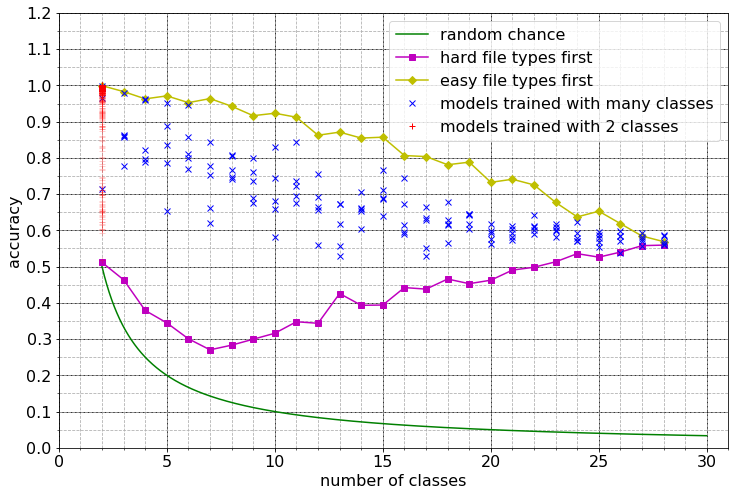
\includegraphics[width=1.0\textwidth]{content/nclasses.png}
\caption{\label{fig:nclasses}Validation accuracy by number of classes}%
\end{figure*}

Figure \ref{fig:dual} shows the graph of the accuracy of each class when compared individually with each one of the others, the 378 possible pairs of classes. File types where all the poins are close to 1.0 are hardly mistaken for other types, while file types presenting some accuracies close to 0.5 can be mistaken for other file types in the perspective of the used model.

\noindent
\begin{figure*}[htb!]
\centering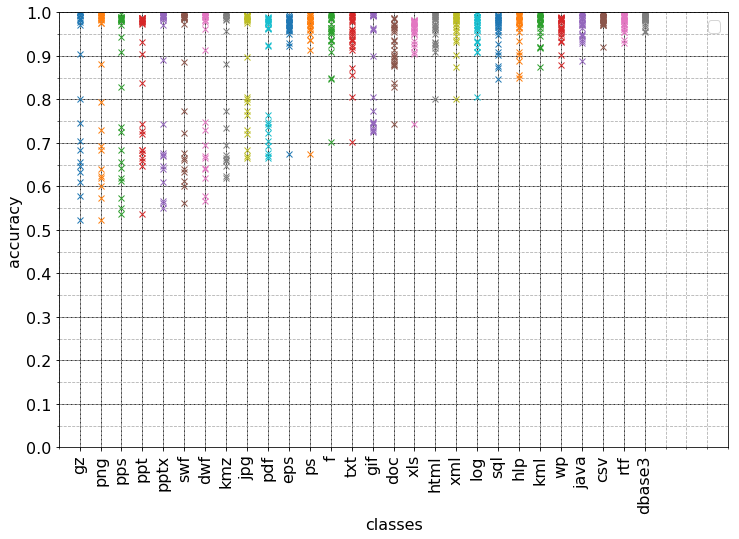
\includegraphics[width=1.0\textwidth]{content/dual.png}
\caption{\label{fig:dual}Validation accuracy of models trained with pair of classes}%
\end{figure*}



A 28x28 matrix was made using the accuracy of the models built for each pair of classes as a distance measure. Then a PCA dimensionality reduction technique was used to plot this data in a 2D graph, grouping similar file types.
The result is shown in figures \ref{fig:pca} and \ref{fig:pca2}. 

\noindent
\begin{figure*}[htb!]
\centering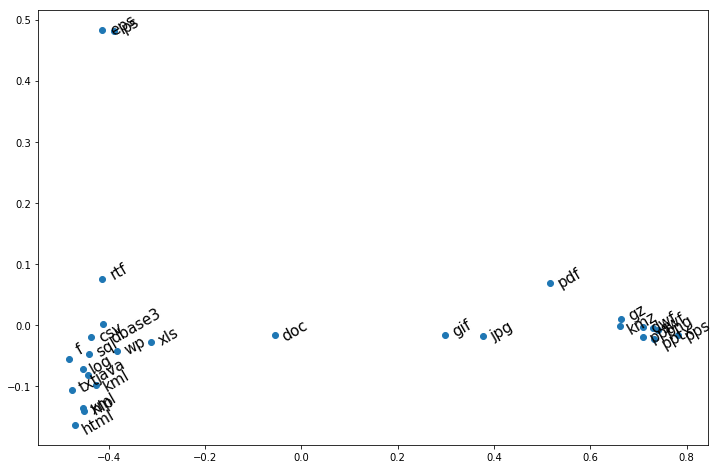
\includegraphics[width=1.0\textwidth]{content/pca.png}
\caption{\label{fig:pca}PCA of accuracy of models trained with pair of classes}%
\end{figure*}


\noindent
\begin{figure*}[htb!]
\centering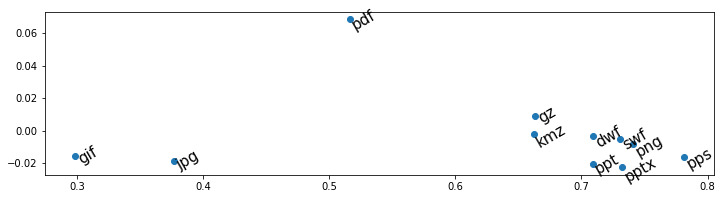
\includegraphics[width=1.0\textwidth]{content/pca2.png}
\caption{\label{fig:pca2}PCA of accuracy of models trained with pair of classes - detail}%
\end{figure*}


% the problem of unseen file types
% \levelC{Limitations and threats to validity}

% \input{content/4.0.3-experimentrandomdata.tex}

%5
\levelA{\label{chap:discussion}Discussion}

%fig 1
\levelB{Accuracy vs. number of classes}

In figure \ref{fig:nclasses}, a decreasing trend was observed. An increase in the number of classes appears to be  correlated with a decrease in accuracy. Another relevant aspect of the graph is that the range of the results seems to be smaller when more classes are used.  

This pattern is understandable: as the number of classes grows, the harder the classification problem is, leading to a decrease in accuracy. Meanwhile, the individual contributions of each class to the overall result diminishes, leading to an increase in precision.

This behavior is an important aspect to consider during the evaluation of file fragments studies. This observation is in agreement with Beebe et al. \cite{beebe_sceadan:_2013} assumption, that studies that select fewer classes tend to yield higher results. 

Still, with 42\% of samples being misclassified when the number of classes is 28, the question of what are the error sources and how they can be addressed requires attention.

The number of possible combinations of file types to compose the datasets depends on the number of classes being considered. For 28 classes there is only one possible combination, while for two classes there are 378. For intermediary values, the numbers are much higher, which is the number of possible combinations disregarding the order of the elements: $ \frac{28!}{(28-n)!n!}$. For 14 file types there are 40116600 combinations. For this reason, the significance of the 5 samples diminishes for intermediary values.

\levelB{Accuracy of pairs of classes}

The accuracy of models trained with pairs of classes, shown in figure \ref{fig:dual}, suggests a reverse correlation between entropy and accuracy.  Generally, file types with higher entropy tend to have lower minima, with the GIF file type being a notable exception. Most of these files use some form of compression, like image files for example.

It was demonstrated that the accuracy of a new model may be manipulated by the selection of file types that will compose the dataset. The lines ``hard file types first'' and ``easy file types first'' of figure \ref{fig:nclasses} were created using the order shown on figure \ref{fig:dual}, resulting in lines that seem to be close to the minimum and maximum of the possible accuracy values. 

\levelB{PCA}

The usage of PCA on the 28x28 distance matrix produced a 2D projection where the file types that use compression or contains images are grouped near each other, as shown in figures \ref{fig:pca} and \ref{fig:pca2}.


    \levelB{Future work}
    compare results with sceadan

 For future researches on file fragment classification, the hypothesis that the remaining 2/3 of the observed errors are caused by similar data structures used by multiple files should be explored. Also, the search for a procedure to automatically label inner data structures of files may be a promising strategy. 

% Having recognized the potential of neural networks in the data carving task, there are still some research paths that should be explored.

% \todo[inline]{qual a dificuldade da tarefa de identificacao do tipo de arquivo, o que os outros metodos atingem de acuracia?}

% \todo[inline]{aumentar número de tipos de arquivos suportados}

% \todo[inline]{Existem aspectos que já avançaram mas não citados no texto, por exemplo, já consegue identificar o início e o fim do arquivo.}

% One of them is about the increase in the range of supported filetypes. In a collaborative approach, should the said community be sharing models, datasets, or both? What are the strengths and weakness of each?

% Another one is about reassembling. After each block has been classified, how to reconstruct the original file in the occurrence of fragmentation?

% \todo[inline]{Quanto a remontagem? Existe uma previsão e qual o dataset tu vais utilizar? Como vai conseguir remontar? Este problema é complicado, mas deve tentar avançar de alguma forma.}

% \todo[inline]{Pretende ainda avançar nos tipos de arquivos e na remontagem. Mesmo que não consiga remontar, pelo menos mostrar o que não conseguiu, pois facilita para quem for feito. —> Verificar a literatura se ninguém está fazendo isto mesmo.}

% The last one is about the recognized structures. Is it possible to use the trained networks to describe the structures being recognized?

% ==========


% The following questions are intended to be answered in future works: 

% \begin{enumerate}[itemindent=\parindent,label=\textbf{Q\arabic*.}]

%     \item Could a neural network based tool support a wider range of file types?
    
%     \item Could a neural network based tool handle fragmentation through reassembling?
    
%     % \item Do the results obtained with usual datasets reflect what happens in real scenarios?

% \item Do neural networks help to interpret internal file structures?

% \end{enumerate}

% \todo[inline]{compare solutions - possible candidates: feedforward, convolutional, LSTM, BLSTM, SVM, kNN, Photorec, Foremost, scalpel}
% \todo[inline]{shuffle data to simulate fragmentation}
% \todo[inline]{removal of portions of files to simulate data corruption}
% \todo[inline]{increase the number of supported file types, investigating the best strategy to scale the solution}
% \todo[inline]{reassembling}
% \todo[inline]{model share}
% \todo[inline]{adaption of visualization techniques of neural networks, attempting to infer file structure.}

\levelA{\label{chap:conclusion}Conclusion}
It was observed that an increase in the number of extensions selected to compose the training had the tendency to decrease accuracy and increase precision. But the number of classes alone is not as important as the type of extension selected: some file types when included in the experiment have a much higher negative impact than others. This observation was demonstrated in the ``hard file types first'' and ``easy file types first'' of figure \ref{fig:nclasses}, where the file types selected to compose  where intentionally chosen, once to degrade results and once to improve them.

File types that contains images or that use compression were identified as those that have the higher negative effect on results, which suggests that their entropy may contribute to the error.

\levelB{Limitations, threats to validity and future work}

The number of samples taken was small when compared with the number of all possible file types combinations. This imposes a limit on the conclusions that can be reached and this limitation is hard to overcome.

The group that emerged as file types that most degrade results are files that use compression or contain images. While they are known for their high entropy, no measure of entropy was used to reinforce this claim. A study is in progress to measure the impact of entropy on file fragment classification errors.

